\scanpage{71}
Groupoïdes de \uline{Teichmüller}

1) Groupoïde topologique. 
\begin{tikzpicture}[baseline=(b.base)]
\node[inner xsep=5pt,inner ysep=4pt] (b) {$S\mathcal T_{\mathrm{top}}$};
\draw (b.north west)--(b.south west)--(b.south east)--(b.north east);
\end{tikzpicture}.
(\uline{groupoïde de Teichmüller spécial orienté topologique})

Objets : paires $(X,S)$
\[
\left|\begin{array}{l}
X\ \text{surface à bord compacte \uline{orientée}}\\
S\subset\partial X\quad\text{partie finie du bord}
\end{array}\right.
\]

Morphismes $(X,S)\longrightarrow(X',S')$ : classes d'isotopie d'isomorphismes

$1^\circ)$ $S=\phi$ on écrit $\mathcal T_{\mathrm{top}}$ sous-groupoïde ouvert.
(\uline{groupoïde de T. \deleted{\unsure{orient|non}} orienté topologique})

\deleted{Vari} \uline{Variantes}
$\unsure{2^\circ|1^\circ})$ 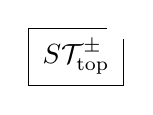
\begin{tikzpicture}[baseline=(b.base)]
\node[inner xsep=5pt,inner ysep=4pt] (b) {$S\mathcal T_{\mathrm{top}}^{\pm}$};
\draw (b.north west)--(b.south west)--(b.south east)--([yshift=-4pt]b.north east);
\draw (b.north west)--([xshift=-6pt]b.north east);
\end{tikzpicture} mêmes objets, mais plus de flèches :
classes d'isotopie d'homéom. $(X,S)\xrightarrow{\sim}(X',S')$, ne respectant pas l'orientation nécessairement.

On a
\diagram{\begin{tikzcd}[ampersand replacement=\&,column sep=large]
S\mathcal T_{\mathrm{top}}^\pm \arrow[r,"\unsure{\chi|\varepsilon|\mathfrak{s}}","\text{(signature}"']
\& \text{\unsure{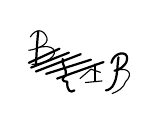
\begin{tikzpicture}[baseline=-.4ex,x=.010cm,y=-.010cm,line cap=round,line join=round]
% Unread cancelled target: visible underlying outlines and cancellation strokes.
\draw[thin] (5,12) .. controls (12,1) and (22,2) .. (26,13)
 .. controls (29,22) and (12,28) .. (3,29);
\draw[thick] (15,5) .. controls (13,24) and (13,35) .. (12,47);
\draw[thin] (14,26) .. controls (34,20) and (42,31) .. (30,40)
 .. controls (23,44) and (16,47) .. (7,47);
\draw[thick] (46,40) .. controls (45,49) and (52,53) .. (50,61)
 .. controls (44,65) and (45,69) .. (52,69)
 .. controls (51,80) and (56,84) .. (61,80);
\draw[thin] (68,65)--(82,53)--(94,57);
\draw[thick] (87,47)--(87,68);
\draw[thin] (75,70)--(96,68);
\draw[thick] (108,45) .. controls (111,31) and (129,29) .. (128,40)
 .. controls (127,50) and (115,55) .. (112,55);
\draw[thick] (117,38) .. controls (115,51) and (116,63) .. (111,72)
 .. controls (109,77) and (104,80) .. (101,80);
\draw[thin] (116,54) .. controls (130,51) and (136,59) .. (126,69)
 .. controls (124,76) and (117,81) .. (109,84);
\draw[thick] (3,45)--(42,27);
\draw[thick] (6,51)--(54,32);
\draw[thick] (12,56)--(69,34);
\draw[thick] (25,59)--(82,41);
\draw[thick] (39,65)--(98,44);
\end{tikzpicture}}}\ \substack{\text{groupoïde \deleted{ponctuel}}\\
\text{défini par le groupe}\\
\pm1,\ \text{noté }[\pm1]}
\end{tikzcd}}

le \deleted{noyau} \deleted{est} (\unsure{la|$=$|en} catégorie fibre) est $S\mathcal T_{\mathrm{top}}$

\figure{\hspace*{4cm}\unsure{
\begin{tikzpicture}[baseline=-.4ex,x=.015cm,y=-.015cm,line cap=round,line join=round]
\draw[line width=1pt] (16,0)--(10,7)--(5,12)--(0,19)
 .. controls (0,25) and (9,31) .. (14,28)
 .. controls (20,25) and (15,15) .. (12,10);
\draw[thick] (7,14) .. controls (2,17) and (3,25) .. (9,27)
 .. controls (15,29) and (19,21) .. (13,20)--(6,15);
\draw[thick] (14,20)--(27,17);
\draw[thin] (5,12)--(12,23);
\fill (30,7)--(31,10)--(36,13)--(33,12)--(29,11)--cycle;
\end{tikzpicture}}}

$2^\circ)$ $(X,\Sigma,S)$, avec
\[
\left|\begin{array}{l}
X\ \text{compacte à bord orienté}\\
\Sigma\ \text{sous-variété \deleted{\unsure{fermée}} \inserted{compacte} de dim $1$}\\
\qquad\text{de }X\setminus\partial X\\
S\subset\Sigma\cup\partial X\quad\text{partie finie}
\end{array}\right.
\]

morphismes : classes d'isotopie d'homéom \unsure{respectant} l'orientation.

Notation $\mathcal T\deleted{\unsure{S}}\inserted{D}_{\mathrm{top}}$

($D$) initiale de.

\deleted{``\unsure{sauvage}''}\inserted{dévissage}) :

``\uline{groupoïde de Teichmüller orienté dévissé topologique}''.

\uline{NB}
\diagram{\begin{tikzcd}[ampersand replacement=\&,column sep=small,row sep=.15em]
S\mathcal T_{\mathrm{top}} \& \subset \& S\mathcal T D_{\mathrm{top}}
\& \substack{\inserted{\text{imm. ouverte}}\\(\deleted{\text{\unsure{inclusion|immersion} pleine}})}\\
\Vert\\
\text{\makebox[0pt][l]{sous groupoïde des objets tels que $\Sigma=\phi$}}
\end{tikzcd}}

$3^\circ)$ On définit de $=$ $\mathcal TS_{\mathrm{top}}^\pm$
(\uline{groupoïde de Teichmüller biorienté dévissé topologique})

\mspage{70}
